% ======================================================
% Compile: xelatex 5state_aprime_kf_meas.tex
% Path:    reference/eq17_analysis/derivation/5state_aprime_kf_meas.tex
% DRAFT (2026-07-20). a' as a PROPER KF state updated by the y2 measurement
% (NOT an external EWMA bolt-on). The residual-gain relation a_r = -a'*dh is
% placed in the MEASUREMENT Jacobian H(2,5), so y2 directly corrects a' via the
% Kalman gain. Route/notation follow 5state_aprime_var_esti.tex; the single
% structural change is Sec.2: a' update = Kalman gain, replacing esti's
% beta-EWMA of a'_hdm. New symbols kept minimal: a_det (desired-height gain),
% DH_d (d-step commanded sweep). y2 g-bias (H(2,4) mirror) EXCLUDED per user.
% ======================================================
\documentclass[11pt,a4paper,fontset=none]{ctexart}

\usepackage[fleqn]{amsmath}
\usepackage{amssymb,bm}
\usepackage{empheq}
\setlength{\mathindent}{0pt}
\usepackage{geometry}
\geometry{margin=2.0cm}
\usepackage{array,booktabs}
\usepackage{graphicx}

\setlength{\parindent}{0pt}
\setlength{\parskip}{0.3em}
\setlength{\abovedisplayskip}{4pt}
\setlength{\belowdisplayskip}{4pt}
\setlength{\abovedisplayshortskip}{2pt}
\setlength{\belowdisplayshortskip}{2pt}

\newcommand{\lc}{\lambda_c}
\newcommand{\ap}{a'}
\newcommand{\aph}{\hat a'}
\newcommand{\adet}{a_{d}}
\newcommand{\adeth}{\hat a_{d}}
\newcommand{\eap}{e_{a'}}
\newcommand{\ead}{e_{a_d}}
\newcommand{\eh}{e_{h}}
\newcommand{\DHd}{\Delta H_d}
\newcommand{\Dh}{\Delta h_d}
\newcommand{\hd}[1]{\par\medskip\noindent\underline{\textbf{#1}}\par\nobreak\vspace{0.2ex}}

\begin{document}

\begin{center}\textbf{\large 5-state EKF: $a'$ as a measured state ($y_2$ update, no bolt-on)}\end{center}
\vspace{-0.4em}
\begin{center}\small DRAFT --- route follows \texttt{5state\_aprime\_var\_esti.tex};
Sec.\,2 replaces the $\beta$-EWMA of $a'_{hdm}$ with a Kalman update of $a'$.\end{center}

\hd{0. Definitions}

\[
h[k] = h_d[k] - \delta h[k], \qquad
\Dh[k] = h_d[k{+}1] - h_d[k], \qquad
\DHd[k] = h_d[k] - h_d[k{-}d]
\]
\[
\adet[k] := a_h\big(h_d[k]\big), \qquad
\ap[k] := \left.\frac{d a_h}{d h}\right|_{h_d[k]}, \qquad
a_r[k] := a_h\big(h[k]\big) - \adet[k]
\]
\[
\delta h[k+1] = \lc\,\delta h[k] - F_{dh}[k]\,\ead[k] - \varepsilon_h[k]
\]
$\adet$ = gain at the desired height (deterministic, trajectory-driven);
$\ap$ = its slope; $a_r$ = residual gain from the tracking error;
$\DHd$ = known $d$-step commanded sweep. $\delta h_1 := \delta h[k{-}d]$ (oldest,
measured), $\delta h_2 := \delta h[k{-}1]$, $\delta h_3 := \delta h[k]$.

\hd{1. True}

First-order Taylor of the gain at the actual (perturbed) height:
\[
a_h\big(h[k]\big) = a_h\big(h_d[k] - \delta h[k]\big)
\approx \adet[k] - \ap[k]\,\delta h[k]
\]

\begin{empheq}[box=\fbox]{equation*}
a_r[k] = -\,\ap[k]\,\delta h[k], \qquad \ap[k+1] \approx \ap[k]
\end{empheq}

The desired-height gain drifts with the commanded sweep:
\begin{empheq}[box=\fbox]{equation*}
\adet[k+1] = \adet[k] + \ap[k]\,\Dh[k]
\end{empheq}

The second measurement reads the \emph{actual} gain $d$ steps ago. Substituting
$\adet[k{-}d] = \adet[k] - \ap\,\DHd[k]$ (from the sweep, $\ap$ slow) and
$\delta h[k{-}d] = \delta h_1$:
\[
y_2[k] = a_h\big(h[k{-}d]\big) = \adet[k{-}d] - \ap\,\delta h[k{-}d] + \nu_2[k]
\]
\begin{empheq}[box=\fbox]{equation*}
y_2[k] = \adet[k] \;-\; \ap[k]\,\big(\DHd[k] + \delta h_1[k]\big) \;+\; \nu_2[k]
\end{empheq}
$a'$ enters $y_2$ \emph{explicitly}, multiplying the total height offset
$\DHd+\delta h_1$ (commanded sweep $+$ thermal tracking error). This is the
relation the var-channel used implicitly; here it is kept as a measurement.

\hd{2. Estimator ($a'$ inside the KF)}

State $\ (5\times1)$:
\[
x = [\,\delta h_1,\ \delta h_2,\ \delta h_3,\ \adet,\ \ap\,]^{\mathsf T}
\]

\textbf{Predict} (deterministic map; $\Dh,\DHd$ known from the trajectory):
\[
\begin{aligned}
\delta h_1[k{+}1] &= \delta h_2[k], &
\delta h_2[k{+}1] &= \delta h_3[k], &
\delta h_3[k{+}1] &= \lc\,\delta h_3[k], \\
\adet[k{+}1] &= \adet[k] + \aph[k]\,\Dh[k], &
\ap[k{+}1] &= \ap[k]. & &
\end{aligned}
\]

\textbf{Measurement} ($y_1$ = delayed position error, $y_2$ = gain gauge):
\[
y_1[k] = \delta h_1[k] + n_x[k], \qquad
y_2[k] = \adet[k] - \ap[k]\big(\DHd[k]+\delta h_1[k]\big) + \nu_2[k]
\]
\[
H_1 = [\,1,\ 0,\ 0,\ 0,\ 0\,]
\]
\begin{empheq}[box=\fbox]{equation*}
H_2[k] = \big[\,-\aph[k],\ \ 0,\ \ 0,\ \ 1,\ \ -\big(\DHd[k]+\delta\hat h_1[k]\big)\,\big]
\end{empheq}

\textbf{Update} (standard EKF; $H=[H_1;H_2]$, $R=\mathrm{diag}(\sigma^2_{n},\,R_2)$):
\begin{empheq}[box=\fbox]{align*}
K[k] &= P^{-}H^{\mathsf T}\big(HP^{-}H^{\mathsf T}+R\big)^{-1}, \qquad
x^{+} = x^{-} + K\big(y - Hx^{-}\big)
\end{empheq}

\textbf{Why $a'$ is now genuinely in the KF.} The gain-row of $K$ is
\[
K_5 = \frac{\big[P^{-}H^{\mathsf T}\big]_5}{S}
    = \frac{P^{-}_{55}\,H_2(5) + P^{-}_{54}\,H_2(4) + \dots}{S},
\qquad H_2(5) = -(\DHd+\delta\hat h_1) \neq 0 .
\]
$a'$ carries its \emph{own} measurement entry $P^{-}_{55}H_2(5)$ (direct
correction), not only the cross-covariance $P^{-}_{54}$. This replaces the esti
recursion $\ap[k{+}1]=\beta\,\ap[k]+(1{-}\beta)\,a'_{hdm}[k]$ (a $\beta$-EWMA of
a variance ratio computed \emph{outside} the filter): $a'$ now updates from the
$y_2$ innovation like any other state.

\hd{3. Error dynamics}

$\eh = \delta h - \delta\hat h$, $\ead = \adet - \adeth$, $\eap = \ap - \aph$.
Predict (before correction):
\[
\ead[k{+}1] = \ead[k] + \Dh[k]\,\eap[k], \qquad
\eap[k{+}1] = \eap[k],
\]
so an $a'$ error feeds the level error at rate $\Dh$ (the sweep coupling).
Linearizing the $y_2$ innovation about the current estimates:
\[
\nu_2 = \ead - \big(\DHd+\delta\hat h_1\big)\,\eap - \aph\,e_{h,1} + \nu_2^{\,\mathrm{noise}} .
\]
The closed loop is the usual EKF contraction
\begin{empheq}[box=\fbox]{equation*}
e[k+1] = \big(I - K[k]H[k]\big)\,F_e[k]\,e[k] + q[k]
\end{empheq}
with $e=[\delta h_1,\delta h_2,\delta h_3,\ead,\eap]^{\mathsf T}$. Because
$H_2(5)\neq0$, the correction $(I-KH)$ acts on $\eap$ \emph{directly} through the
$y_2$ innovation --- the mechanism the bolt-on lacked.

\hd{4. $\mathbf F_e$ and $\mathbf H$}

\[
F_e[k] =
\begin{bmatrix}
0 & 1 & 0 & 0 & 0 \\
0 & 0 & 1 & 0 & 0 \\
0 & 0 & \lc & -F_{dh}[k] & 0 \\
0 & 0 & 0 & 1 & \Dh[k] \\
0 & 0 & 0 & 0 & 1
\end{bmatrix},
\qquad
H[k] =
\begin{bmatrix}
1 & 0 & 0 & 0 & 0 \\
-\aph[k] & 0 & 0 & 1 & -\big(\DHd[k]+\delta\hat h_1[k]\big)
\end{bmatrix}
\]
Time-varying entries: $F_e(3,4)=-F_{dh}[k]$, $F_e(4,5)=\Dh[k]$ (sweep coupling,
predict), and the whole of $H_2[k]$ (measurement coupling). Row $5$ of $F_e$ is a
pure integrator; $a'$ acquires dynamics only through the measurement, not a
process pole.

\hd{5. Observability and caveats}

\textbf{Two channels in one entry.}
$H_2(5) = -(\DHd+\delta\hat h_1)$: the commanded sweep $\DHd$ (deterministic,
present only in motion) and the thermal tracking error $\delta\hat h_1$
(stochastic, present in holds). Both routes to $a'$ live in the single
measurement entry.

\textbf{Bilinear EKF.} $y_2$ contains the product $\ap\,\delta h_1$; both
$H_2(1)=-\aph$ and $H_2(5)=-(\DHd+\delta\hat h_1)$ come from it, so $a'$ and
$\delta h_1$ are coupled in the same measurement. Identifiability (does an
innovation load onto $\eap$ or $e_{h,1}$?) is set by the covariance and must be
checked --- in a pure hold ($\DHd=0$) both are read from the same thermal product.

\textbf{Hold floor unchanged.} $\DHd=0 \Rightarrow H_2(5)=-\delta\hat h_1$, so
$a'$ observability scales with the thermal amplitude $\sim\!\sqrt{\mathrm{Var}(\delta h)}$
over a finite dwell --- a CRLB floor, independent of this reformulation.

\textbf{Not self-referential.} $y_2=a_{xm}$ is a real measurement carrying
$-\ap_{\mathrm{true}}\,\delta h$; the innovation delivers genuine truth to $a'$,
unlike the var-channel's self-constructed $\hat a_r$ (which returns $\aph$).

\hd{6. Process / measurement noise ($Q$, $R$) and the closed loop}

Predict noise $Q=\mathrm{diag}(0,0,Q_{33},Q_{44},Q_{55})$ (rows $1,2$ are pure
delays), measurement noise $R=\mathrm{diag}(R_1,R_2)$ on $(y_1,y_2)$. Four of the
five nonzero entries are fixed by first principles; only $Q_{55}$ carries a design
choice (Option~A below).

\textbf{$Q_{33}$ --- thermal drive of $\delta h_3$.} The white term in
$\delta h_3[k{+}1]=\lc\,\delta h_3[k]-F_{dh}\ead-\varepsilon_h[k]$ is the thermal
position increment $a\,f_T$ over one step. With
$\mathrm{Var}(f_T)=4k_BT\,\gamma_N/\Delta t$ and $a=\Delta t/\gamma_N$,
\[
\mathrm{Var}(\varepsilon_h)=a^2\,\mathrm{Var}(f_T)=4k_BT\,\tfrac{\Delta t}{\gamma_N}=4k_BT\,a .
\]
\begin{empheq}[box=\fbox]{equation*}
Q_{33}=4k_BT\,\adeth
\end{empheq}
(fluctuation--dissipation; evaluated at the estimated gain $\adeth$).

\textbf{$R_1$ --- $y_1$ sensor noise.} $y_1=\delta h_1+n_x\Rightarrow R_1=\sigma^2_{n}$.

\textbf{$R_2$ --- $y_2=a_{xm}$ gauge noise.} $a_{xm}$ is the IIR variance-ratio gain
gauge (paper 2025, Eq.\,9--13); its linear-inversion readout noise was derived as a
quadratic in the gain,
\begin{empheq}[box=\fbox]{equation*}
R_2=a_{cov}\,\mathrm{IF}_{var}\,\big(\adeth+\xi\big)^2,\qquad
\xi=\frac{C_n}{C_{dpmr}}\,\frac{\sigma^2_{n}}{4k_BT},
\end{empheq}
with $C_{dpmr}=2+\tfrac{1}{1-\lc^2}\approx3.96$, $C_n=\tfrac{2}{1+\lc}\approx1.18$,
$\mathrm{IF}_{var}\approx4.24$ ($\lc=0.7$, Option~A autocorrelation). \emph{No}
delay-transport ($+5Q_{77}$) term is needed: the $d$-step delay is carried
explicitly by $\DHd$ inside $H_2$, not by an inflated $R_2$.

\textbf{$Q_{44}$ --- $a_d$ (structural, $\approx0$).} The predict
$\adet[k{+}1]=\adet[k]+\aph\,\Dh$ is first-order exact. Its two residuals are
(i) the gain-estimate error $(\ap-\aph)\Dh$, routed through $\eap$ by
$F_e(4,5)=\Dh$ (\emph{not} process noise), and (ii) the Taylor truncation
$\tfrac12 a''\Dh^2$, the only genuine model noise:
\begin{empheq}[box=\fbox]{equation*}
Q_{44}=\big(\tfrac12\,a''\,\Dh^2\big)^2\approx0
\qquad(\Dh=O(v_d\Delta t)\ \text{per step}) .
\end{empheq}
There is deliberately \emph{no} $(\aph)^{2}Q_{33}$ term: the thermal gain wander lives
in the reconstruction $\hat a_z=\adet-\aph\,\delta\hat h_3$ (a deterministic function of
the state $\delta h_3$), not in the $a_d$ process noise --- this is the $\sim\!30\times$
predict-side reduction over the leak-free-integrator gain state.

\textbf{Caveat (code vs derivation, 2026-07-22).} The temp harness currently runs
$Q_{44}=(\aph)^{2}Q_{33}$ (the taylor gain-wander, a leftover from the
slot-4$=$actual-gain parametrization), \emph{not} this $\approx0$ form --- i.e.\ the
thermal wander is double-counted (once here, once in the reconstruction). Whether
$Q_{44}\approx0$ (this derivation) or $(\aph)^{2}Q_{33}$ (code) is correct is
\emph{unresolved}: the $a'$-uncertainty is already propagated into $P_{44}$ by
$F_e(4,5)=\Dh$, which argues for $\approx0$. All \S8/\S9 numbers were run on the
code's $(\aph)^{2}Q_{33}$.

\textbf{$Q_{55}$ --- $a'$ (Option~A).} $a'$ is the slope \emph{at the desired
height} $h_d$, so it drifts only with the commanded sweep --- no thermal term:
\[
w_{a'}[k]=\ap[k{+}1]-\ap[k]=a''(h_d)\,\Dh[k]
\quad\Longrightarrow\quad
Q_{55}[k]=\big(a''\,\Dh[k]\big)^2 .
\]
\emph{Hold} ($\Dh=0$): $Q_{55}=0$ \emph{exactly} --- $a'$ is genuinely constant,
$P_{55}$ does not inflate from process noise, and the cap/gate that a flat $Q_{55}$
would demand is unnecessary. The low-excitation hold is handled by the model, not an
external switch.
\begin{empheq}[box=\fbox]{equation*}
Q_{55}\big|_{\text{hold}}=0,\qquad
Q_{55}\big|_{\text{motion}}=\big(a''\,\Dh\big)^2 .
\end{empheq}
\emph{Motion:} $(a''\Dh)^2$ needs $a''$, unknown (second derivative of the unknown
$c(\bar h)$). \textbf{Option~A} takes $a''\!\approx\!0\Rightarrow Q_{55}\!\approx\!Q_{55}^{\min}$
(a small floor keeping the channel alive); $a'$ is then a constant state driven only by
the $y_2$ (and forthcoming $y_3=\delta x_{md}$) innovations. Zero assumption on $c$; if
a fast descent shows $a'$ lag, escalate to adaptive $\hat a''\approx\Delta\aph/\Dh$
(Option~B) or an $a_d$-curvature bound (Option~C).

\hd{7. Identifiability and the closed loop}

$y_2$ carries the product $\ap\,\delta h_1$; $H_2(1)=-\aph$ and
$H_2(5)=-(\DHd+\delta\hat h_1)$ both come from it, so $a'$ and $\delta h_1$ share the
$y_2$ innovation and the split is set by $P^-$. In a pure hold ($\DHd=0$) both are read
from the same thermal product, so $a'$ observability scales as
$\sqrt{\mathrm{Var}(\delta h)}$ over the dwell --- a CRLB floor. This floor \emph{is} the
model's own gentle behaviour: $K_5\propto P_{55}H_2(5)\to0$ as $\DHd\to0$ and
$Q_{55}\to0$, i.e.\ the ``no gate'' mechanism written in equations.

The closed loop is
\[
e[k{+}1]=\big(I-K[k]H[k]\big)F_e[k]\,e[k]+q[k],\qquad
e=[\delta h_1,\delta h_2,\delta h_3,\ead,\eap]^{\mathsf T},
\]
with $Q=\mathrm{diag}(0,0,Q_{33},Q_{44},Q_{55})$ and $R=\mathrm{diag}(R_1,R_2)$. Under
Option~A ($Q_{44},Q_{55}\!\to\!$ floor) the steady state solves the discrete
Lyapunov/Riccati recursion; $P_{55}^{ss}$ is the $a'$ variance floor and, through
$\hat a_z=\adet-\aph\,\delta\hat h_3$, sets the $\hat a_z$ floor. The full symbolic solve
is deferred to the integration step (block~D, with the deterministic channel
$y_3=\delta x_{md}$ added), since $y_3$ changes the $a_d/a'$ observability.

\hd{8. Verification (Option~A, 1\,Hz canonical, pure-MATLAB)}

Setup: $\bar h$ swept $22\!\to\!2$ over hold $0.5$\,s $\to$ descent $1$\,s $\to$
four $1$\,Hz cycles ($T=6$\,s), thermal $+$ measurement noise on, seed~1
($+\,6$-seed robustness). $Q_{55}=$ Option~A ($a''\!\approx\!0$, floor
$10^{-12}$); the baseline reference is the $\kappa$-model
$Q_{55}=\kappa^2(\aph)^2\Dh^2/(h_d\!-\!h_w)^4$ (which implicitly assumes
$a''\!\sim\!\kappa\,a/(h_d\!-\!h_w)^2$, a mild $c$-form). Estimate
$\hat a_z=\adet-\aph\,\delta\hat h_3$.

\begin{center}\small
\begin{tabular}{lccc}
\toprule
metric & Option~A & baseline $\kappa$ & oracle ($a'$ known) \\
\midrule
first-hold std$(\hat a_z)$ [nm/pN]    & $0.021$ & $0.022$ & $0.015$ \\
osc rel.\ err $(\hat a_z)$            & $6.5\%$ & $5.6\%$ & $2.3\%$ \\
osc corr$(a',a'_{\mathrm{oracle}})$  & $\approx0$ & $\approx0$ & --- \\
$\max|a'|$ (6 seeds)                  & $<4\!\times\!10^{-3}$ & $<4\!\times\!10^{-3}$ & --- \\
\bottomrule
\end{tabular}
\end{center}

\begin{center}
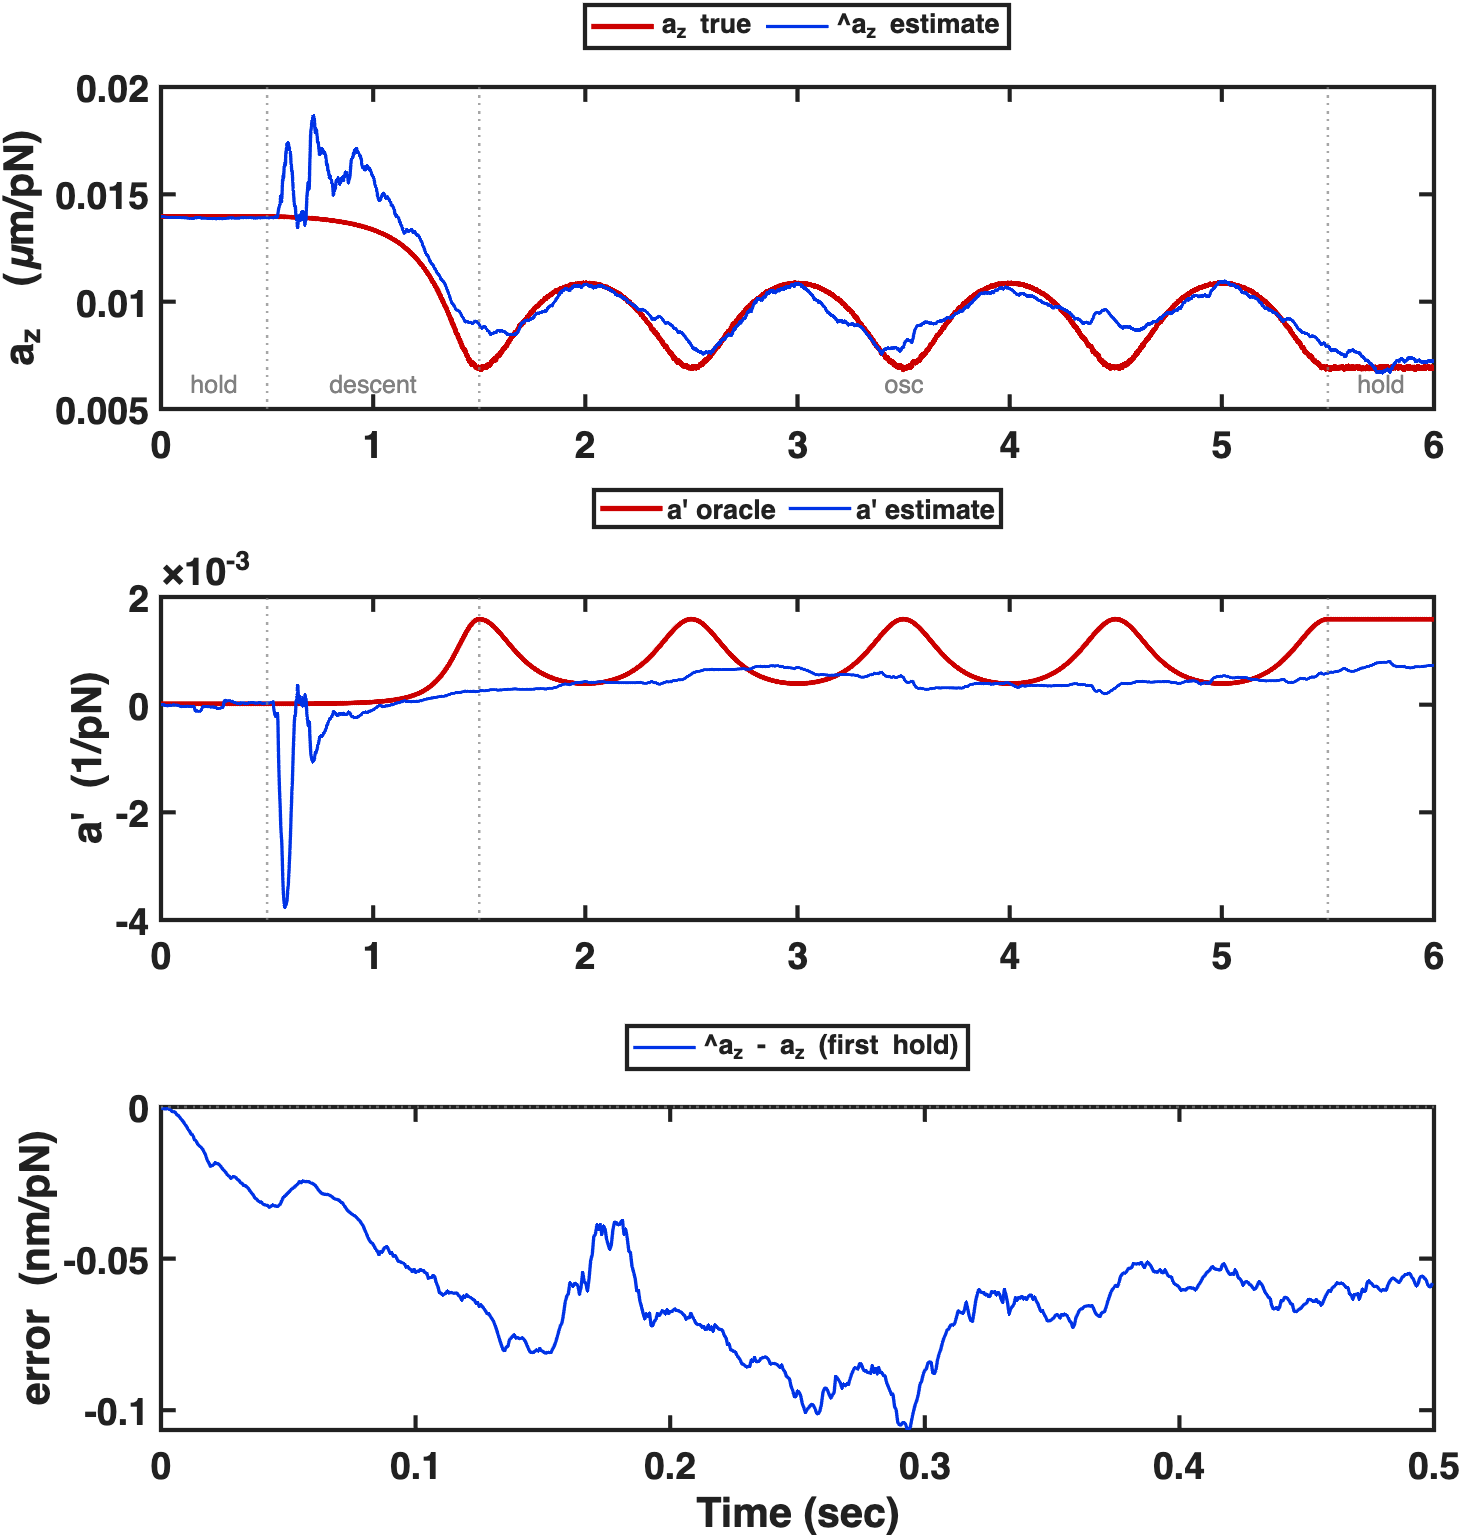
\includegraphics[width=0.92\textwidth]{figures/kfmeas_optA_verify.png}
\end{center}
\vspace{-0.6em}
{\small Top: gain $\hat a_z$ (blue) vs $a_z$ true (red). Middle: $a'$ estimate vs
oracle. Bottom: first-hold error $\hat a_z-a_z$ ($<0.1$ nm/pN).}

\textbf{Confirmed.} \emph{(i)} First-hold $\hat a_z$ is clean
($0.021\!\approx\!0.015$ nm/pN, \emph{no gate}): with $\Dh=0$ the $a_d$ predict
freezes and $Q_{55}=0$, so $P_{55}$ does not inflate and $a'$ stays near its
(correct) $\approx0$ --- the ``no gate'' claim of \S6--7 realized. \emph{(ii)} No
catastrophic blow-up across $6$ seeds ($\max|a'|<4\!\times\!10^{-3}$); the earlier
reported $a'\!\to\!-24$ was a sporadic first-run EKF fragility, not reproduced.
\emph{(iii)} Option~A (charter-clean, $a''\!\approx\!0$) is marginally smoother but
$\sim\!1\%$ less accurate than the $\kappa$-model (charter-questionable); Option~A
is kept.

\textbf{Two residuals (open).}
\emph{(a) Descent-onset transient} --- at the descent start $a'$ over-corrects once
($\to-3.8\!\times\!10^{-3}$), so $\hat a_z$ overshoots $\sim\!30\%$ for
$\sim\!0.4$\,s then recovers (bounded, transient phase). Cause: $P_{55}$ is held at
its prior through the info-starved hold, then dumped by the first strong descent
innovation. Fix is a rate-limit on $a'$ or a smaller $P_{55}^{0}$ (\emph{not} a
gate). \emph{(b) Osc accuracy floor} --- $\hat a_z$ osc error $6.5\%$ vs oracle
$2.3\%$, and $a'$ itself is not tracked (osc corr $\approx0$): the single gain
gauge $a_{xm}$ is too noisy to pin $a'$ under fast motion. Breaking this needs the
independent deterministic channel $y_3=\delta x_{md}$ (C2, block~C), not a $Q/R$
retune.

\hd{9. The deterministic channel $C_2$ ($y_3=\delta x_{md}$, level measurement)}

\textbf{The discarded half.} The tracking error splits as
$\delta x_m=\delta x_{md}+\delta x_{mr}$ --- a deterministic (systematic) part and a
random (thermal) part. The gauge $y_2=a_{xm}$ uses only $\mathrm{Var}(\delta x_{mr})$,
throwing $\delta x_{md}$ away. $C_2$ recovers it as an \emph{independent} measurement.

\textbf{Mechanism.} The controller applies $f_d=(1/\hat a_z)\{\cdots\}$ with the
reconstructed gain $\hat a_z=\adeth-\aph\,\delta\hat h_3$; a gain mismatch injects a
deterministic forcing, and the systematic error obeys (Sec.\,0)
\[
\delta x_{md}[k{+}1]=\lc\,\delta x_{md}[k]-F_{dh}[k]\,(a-\hat a_z)+O(e^2),
\qquad F_{dh}[k]=f_d[k]+(1{-}\lc)\!\sum_i f_d[k{-}i] .
\]
To first order the reconstruction error is the \emph{level} error,
$a-\hat a_z=(\adet-\adeth)-(\ap\,\delta h-\aph\,\delta\hat h_3)=\ead+O(e^2)$ (the
$a'$ term is a product of errors), so $C_2$ measures the level state $\adet$.
$F_{dh}$ (the applied control force) is known and $c$-free --- and is exactly the
$F_e(3,4)$ coupling already in the model.

\textbf{Extraction $\to$ measurement} (parallel to $y_2$): low-pass both sides and
solve for the level error,
\begin{empheq}[box=\fbox]{equation*}
y_3[k]:=\delta x_{md}[k{+}1]-\lc\,\delta x_{md}[k]=-F_{dh}[k]\,\ead[k]+\nu_3[k],
\qquad z_3:=\adeth-\frac{y_3}{F_{dh}}=\adet .
\end{empheq}
$z_3$ is a direct, $c$-free measurement of the true desired-height gain:
\[
H_3=[\,0,\ 0,\ 0,\ 1,\ 0\,]\ (\text{on }\adet),\qquad
\kappa_{C_2}:=\text{recovery efficiency}\approx0.90\text{--}0.94\ (\text{unbiased}) .
\]
Where $y_2$ reads the \emph{delayed} gain through a variance
($H_2=[-\aph,0,0,1,-(\DHd+\delta\hat h_1)]$), $y_3$ reads the \emph{current level}
through the deterministic residual --- a physically independent route.

\textbf{$R_3$ (route~C: white).}
\begin{empheq}[box=\fbox]{equation*}
R_3[k]=\frac{\sigma^2_{\nu_3}}{F_{dh}^2[k]},\qquad
|F_{dh}[k]|<F_{\min}\ \Rightarrow\ R_3\to\infty\ (\text{gate off}) .
\end{empheq}
$\nu_3$ is the random part $\delta x_{mr}$ leaking through the finite-window
low-pass. Verified floor: one $W$-window recovers $\adet$ to $\sim\!9.4\%\,a$ at
$W=0.5$\,s ($\sim\!1/\sqrt W$), and to $6.2\%\,a$ in the descent (single-direction
excitation --- the golden segment); a hold is uninformative ($\sim\!26\%$ at low
force), handled by the $F_{\min}$ gate. Route~C books $\nu_3$ white; it is in fact
EWMA-coloured (same family as coloured-$a_{xm}$), deferred to an AR(1) honesty pass
if $P_{44}$ over-confidence shows.

\textbf{Why it passes the $a_{xm}$ floor.} $\nu_3$ (deterministic-residual
extraction) is independent of the $y_2$ noise (variance-ratio), so two gain
measurements combine as $1/\sigma^2=1/\sigma^2_{y_2}+1/\sigma^2_{y_3}$. They are
time-complementary: the descent/oscillation, where $a_{xm}$ is noisiest, is exactly
where $y_3$ is sharpest, so the combined level variance drops below the
$a_{xm}$-only floor. In a hold both channels gate off (no excitation) --- consistent
with the CRLB, no free lunch.

\textbf{Caveats.} \emph{(i) Endogeneity}: $F_{dh}$ must be the deterministic applied
force $F_{dh}^{\det}$ (low-passed), not the instantaneous $f_d$, or $y_3$ correlates
with its own noise and biases. \emph{(ii) Slow}: window-integrated ($0.5$--$1$\,s),
$\ge4$ windows for $5\%$ --- a level trimmer, not a per-step corrector.
\emph{(iii) Honesty}: the white $R_3$ is provisional (route~C); check $P_{44}$ before
trusting the gain-error bar.

\textbf{Verification (route~C, 1\,Hz canonical, pure-MATLAB).} Adding $y_3$ to the
Option-A filter (per-step, white $R_3$) cuts the descent rel.\ error of $\hat a_z$
from $12.2\%$ to $6.1\%$ (halved, robust across seeds) --- the previously worst
segment. The oscillation improves only modestly ($8.5\%\!\to\!7.5\%$): there $F_{dh}$
oscillates through zero and the residual weakens (prior $C_2$: descent $100\%$ vs osc
$85$--$93\%$ alive). A block \emph{multi-window} weighted-LS was tested and
\emph{rejected} --- monotonically worse as the window grows (both segments), because
the per-step update with $R_3\propto F_{dh}^{-2}$ \emph{already is} recursive weighted
least-squares: the Kalman recursion auto-down-weights the zero-crossings, and an
explicit window only adds staleness ($a_d$ drifts within it) and fewer updates.
Per-step is C2's optimal form; the osc floor is its genuine limit, not a tuning
artefact.

\end{document}
